\chapter{Numerical methods for evolution problems - Stability}
As seen previously, evolution problems concern is the stability of the forward substitution. We will introduce the subject on ordinary differential equations since after discretization a partial differential equation is transformed into a system of ordinary differential equations. We are going to consider model equations for hyperbolic and parabolic equations which will be respectively advection and diffusion equations: 

\begin{equation}
\frac{\D u}{\D t} + \underbrace{a}_{\mbox{or } u} \frac{\D u}{\D x} = 0 \qquad \frac{\D u }{\D t} = \alpha \frac{\D ^2u}{\D x^2}
\end{equation}

\section{Consistency - stability - convergence}
Convergence is a concept we have introduced before, the numerical method is convergent if $\lim _{h\rightarrow 0} || u^h - u|| = 0$ when the number of parameters tends towards infinity, where $u^h$ is the approximate numerical solution and $u$ the exact solution and $h$ is representative of the mesh size. For methods based on a functional representation (finite elements, spectral methods), convergence can be proven directly using functional analysis, see literature. When it is time dependent problem, we use finite differences for time integration (we don't need flexibility for time it is uniform). Finite differences convergence cannot be proven directly, but in contrasts is proven indirectly using the concept of consistency and stability. 

\subsection{Consistency}
We say that a numerical method is consistent if $\lim _{h\rightarrow 0} ||D^h(u^h) - D(u)||=0$ when the mesh size tends towards 0, where $D(u)$ is the differential operator applied to exact solution and the other discrete approximation of the differential operator. That's nothing else but the truncation error.  For example if the problem was: 

\begin{equation}
\frac{\D u}{\D x} = f \qquad \frac{u_{i+1}-u_{i-1}}{2h} = f_i \qquad
 \underbrace{\Rightarrow}_{+} \frac{u_{i+1}-u_{i-1}}{2h} - \left( \frac{\D u}{\D x}\right) _i + f_i - f_i = TE = \mathcal{O}(\Delta x^2)
\end{equation}

which shows that we have indeed the truncation error. For ODE the truncation error only depends on the mesh size $\mathcal{O}(h^p)$, so we need at least a first order accurate $p\leq 1$ method. For PDE, this depends on the mesh spacing in all variables under various combinations, and sometimes it is imposed to be consistent. Consider for example the advection equation

\begin{equation}
\frac{\D u}{\D t} + a\frac{\D u }{\D x} = 0
\end{equation}

The Lax-Friedrichs method gives: 

\begin{equation}
\begin{aligned}
&\frac{u_i^{n+1}-\frac{1}{2}(u_{i-1}^n+u_{i+1}^n)}{\Delta t} + a \frac{u_{i+1}^n - u_{i-1}^n}{2\Delta x} = 0 \\ 
\mbox{but } &\left\{
\begin{aligned}
&u_{i+1}^n = u_i ^n + \Delta x \left(\frac{\D u}{\D x} \right)^n_i + \frac{\Delta x^2}{2} \left.\frac{\D ^2 u}{\D x^2} \right|^n_i + \frac{\Delta x^3}{6} \left.\frac{\D ^3 u}{\D x^3} \right|^n_i\\
&u_{i}^{n+1} = u_i ^n + \Delta t \left(\frac{\D u}{\D t} \right)^n_i + \frac{\Delta t^2}{2} \left.\frac{\D ^2 u}{\D t^2} \right|^n_i
\end{aligned}
\right.\\
\Rightarrow &\frac{\Delta t \left(\frac{\D u}{\D t} \right)^n_i + \frac{\Delta t^2}{2} \left.\frac{\D ^2 u}{\D t^2} \right|^n_i - \frac{\Delta x^2}{2} \left.\frac{\D ^2 u}{\D x^2} \right|^n_i + \dots}{\Delta t} + a \left( \left.\frac{\D u}{\D x}\right|^n_i + \left.\frac{\Delta x^2}{3} \frac{\D ^3 u }{\D x^3}\right|^n_i  + \dots \right) \\
&= \left(\frac{\D u }{\D t} \right)^n_i + a \left(\frac{\D u}{\D x}\right)^n_i + \frac{\Delta t }{2} \frac{\D ^2 u}{\D t^2} - \frac{\Delta x^2}{2\Delta t} \frac{\D ^2 u}{\D x^2} + \dots
\end{aligned}
\end{equation}

We see that when $\Delta t \rightarrow 0$, the first term is 0 but the second one is 0 only if $\lim _{\Delta t, \Delta x \rightarrow 0}(\Delta x^2 /\Delta t) = 0$. 

\subsection{Stability}
Following Lax's definition, a numerical method is said to be stable if the numerical solution in a value T of the evolution variable t remains bounded as the mesh size $\Delta t \rightarrow 0$. For ODE: 

\begin{equation}
\lim _{\Delta t \rightarrow 0, n \rightarrow \infty, n\Delta t = T} u ^n \mbox{ exists}
\end{equation}


\subsection{Convergence}
A numerical method is said to be convergent if: 

\begin{equation}
\lim _{h\rightarrow 0} (u - u^h) = 0
\end{equation}

We prove convergence from consistency and stability using Lax's equivalence theorem: \\

\theor{
\textbf{Lax's equivalence theorem}\\

For a well posed initial value problem and a consistent discretization method, stability is the necessary and sufficient condition for convergence: 

$$ \mbox{Consistency + Stability } \Leftrightarrow \mbox{ Convergence} $$
}

\section{Spectrum of the space discretization - Fourrier analysis}
If we start from a PDE and we discretize all the variables except the evolution variables, we get a system of ODE's: 

\begin{equation}
\frac{d U}{d t} = F(U)
\end{equation}

If the PDE is linear, and if the discretization formula is linear, then this system is linear as well: 

\begin{equation}
\frac{d U}{dt} = SU + Q
\end{equation}

where $U$ is an n vector and $S$ is an $n\times n$ matrix ($n$ is the number of degrees of freedom). So far all the discretization methods we discussed, have been linear, for example: 

\begin{equation}
\frac{\D u}{\D x} \approx \frac{u_{i+1}+u_{i-1}}{2\Delta x}
\end{equation}

because if we replace $u$ by a combination of u and v we will have a linear combination. It turns out that for hyperbolic problems and in particular for non-linear ones, linear discretization will produce purely oscillatory solutions, except in first order. It has been discovered that it was possible to go beyond first order discretization without oscillatory solution but this is not viewed in the frame of this course. \\

If we assume that the matrix $S$ has a complete set of eigenvalues and eigenvectors (real or complex) then we know that the matrix can be diagonalized such that $LS = \Lambda L$:

\begin{equation}
L\frac{dU}{dt} - LSU = LQ \Leftrightarrow L\frac{dU}{dt} - \Lambda LU = LQ \qquad \Rightarrow \frac{dw_i}{dt} - \lambda ^{(i)}w_i = (LQ )_i 
\end{equation}

which gives a set of uncoupled equations, model equations. This allows to separately study the stability of time integration for each mode, that depends on the eigenvalue spectrum of the matrix $S$ resulting from the space discretization of the differential operator. Finding the space discretization is complex because depends on the PDE and the discretization. However, some analytic results have been obtained for some model problems.

\subsection{Spectrum of the central space discretization of the diffusion equation}
The equation we want to look at is the model of parabolic equations (diffusion equation):
\begin{equation}
\frac{\D u}{\D t} = \alpha \frac{\D ^2 u}{\D x^2}
\end{equation}

where $\alpha $ is the diffusivity coefficient [$L^2T^{-1}$]. The evolution parameter is $t$, we want to discretize the equation by central finite differences on a mesh of $N+1$ points in the interval $0 \leq x \leq L$ (so $\Delta x = L/N$). The discretization of an internal point ($1\leq i \leq N-1$) is: 

\begin{equation}
\frac{d u _i}{d t} = \alpha \frac{u_{i+1}-2u_i + u_{i-1}}{\Delta x^2}
\label{3.12}
\end{equation}

We will consider 3 problems varying from boundary conditions. We have to impose an initial condition on one boundary at left and right boundary. 

\subsubsection{Dirichlet conditions} 

Here $u(0,t) = u_0(t) = a, u(N,t) = u_N(t) = b$ are specified. These can easely be eliminated by having the following system for the remaining $N-1$ points: 

\begin{equation}
\frac{d}{dt} \left(\begin{array}{c}
u_1\\
u_2 \\
\vdots\\
u_{N-2}\\
u_{N-1}
\end{array} \right) = \frac{\alpha }{\Delta x^2}
\left(
\begin{array}{ccccc}
-2 & 1  \\
1 & -2 & 1  \\
& \ddots & \ddots & \ddots \\
&  & 1 & -2 & 1\\
& & & 1& -2
\end{array}
\right)\left(\begin{array}{c}
u_1\\
u_2 \\
\vdots\\
u_{N-2}\\
u_{N-1}
\end{array} \right)
+
\left(\begin{array}{c}
\frac{\alpha u_0}{\Delta x^2}\\
0\\
\vdots\\
0\\
\frac{\alpha u_N}{\Delta x^2}
\end{array} \right)
\end{equation}

The eigenvalues are (not detailed in the course): 

\begin{equation}
\lambda ^{(j)} = \frac{-4\alpha}{\Delta x^2}\sin ^2 \left( \frac{\pi j}{2N} \right) \qquad j = 1,\dots ,N-1
\end{equation}

Notice that they are all negative reals and they span a very large range, the first Fourrier mode corresponds to a wave of wavelength $2L$:

\begin{equation}
\begin{aligned}
&\lambda _{1} = -\frac{4\alpha}{\Delta x^2} \sin ^2 \frac{\pi}{2N} \approx - \frac{4\alpha}{\Delta x^2} \left( \frac{\pi}{2N} \right)^2 = - \frac{\alpha}{L^2}\pi ^2\\
&\lambda _{N-1} = -\frac{4\alpha}{\Delta x^2} \sin ^2 \frac{\pi (N-1)}{2 N}\approx \frac{-4 \alpha}{\Delta x^2} 
\end{aligned}
\end{equation}

\subsubsection{Neumann conditions at the left end and Dirichlet at the right end}
 $\left.\frac{\D u}{\D x}\right|_0 = a, u_N$ specified, we have to express the discretization of the left boundary point (i = 0). This can be done like: 

\begin{equation}
\begin{aligned}
&\frac{d u _0}{dt} = \frac{\alpha}{\Delta x^2} (u_1 -2u_0 + u_{-1}) = \frac{\alpha }{\Delta x^2}(2u_1 - 2 u_0) - \frac{2\alpha a}{\Delta x}\\
&\left. \frac{\D u}{\D x}\right|_0 = \frac{u_1 - u_{-1}}{2\Delta x} = a \Rightarrow u_{-1} = u_1 - 2a \Delta x
\end{aligned}
\end{equation}

So that here we have $N$ unknowns, and only the first line changes:

\begin{equation}
\frac{d}{dt} \left(\begin{array}{c}
u_0\\
u_1 \\
\vdots\\
u_{N-2}\\
u_{N-1}
\end{array} \right) = \frac{\alpha }{\Delta x^2}
\left(
\begin{array}{ccccc}
-2 & 2  \\
1 & -2 & 1  \\
& \ddots & \ddots & \ddots \\
&  & 1 & -2 & 1\\
& & & 1& -2
\end{array}
\right)\left(\begin{array}{c}
u_0\\
u_1 \\
\vdots\\
u_{N-2}\\
u_{N-1}
\end{array} \right)
+
\left(\begin{array}{c}
-\frac{2\alpha a}{\Delta x}\\
0\\
\vdots\\
0\\
\frac{\alpha u_N}{\Delta x^2}
\end{array} \right)
\end{equation}

The eigenvalues are: 

\begin{equation}
\lambda ^{(j)} = \frac{-4\alpha}{\Delta x^2}\sin ^2 \left( \frac{(2j-1)\pi}{4N} \right) \qquad j = 1, \dots , N
\end{equation}

The first Fourrier mode is now a wave with wavelength = $4L$:

\begin{equation}
\begin{aligned}
&\lambda _{1} = -\frac{4\alpha}{\Delta x^2} \sin ^2 \frac{\pi}{4N} \approx - \frac{4\alpha}{\Delta x^2} \left( \frac{\pi}{4N} \right)^2 = - \frac{\alpha}{4L^2}\pi ^2\\
&\lambda _{N} = -\frac{4\alpha}{\Delta x^2} \sin ^2 \frac{\pi (2N-1)}{4 N}\approx \frac{-4 \alpha}{\Delta x^2} 
\end{aligned}
\end{equation}


\subsubsection{Periodic boundary conditions}
Now $u_0 = u_N$ and the system is 
\begin{equation}
\frac{d}{dt} \left(\begin{array}{c}
u_0\\
u_1 \\
\vdots\\
u_{N-2}\\
u_{N-1}
\end{array} \right) = \frac{\alpha }{\Delta x^2}
\left(
\begin{array}{ccccc}
-2 & 1& & & 1  \\
1 & -2 & 1  \\
& \ddots & \ddots & \ddots \\
&  & 1 & -2 & 1\\
1 & & & 1& -2
\end{array}
\right)\left(\begin{array}{c}
u_0\\
u_1 \\
\vdots\\
u_{N-2}\\
u_{N-1}
\end{array} \right) 
+
\left(\begin{array}{c}
0\\
0 \\
\vdots\\
0\\
0
\end{array} \right) 
\end{equation}

The eigenvalues are: 

\begin{equation}
\lambda ^{(j)} = \frac{-4\alpha}{\Delta x^2}\sin ^2 \left( \frac{\pi j}{N} \right) \qquad j = 0, \dots, N-1
\end{equation}

Since the system has $N$ unknowns, it has $N$ eigenvalues, the first one is zero since the system matrix is singular. The first to be non zero is the first Fourrier mode of wavelength $L$: 

\begin{equation}
\begin{aligned}
&\lambda _{0} = 0\\
&\lambda _{1} = -\frac{4\alpha}{\Delta x^2} \sin ^2 \frac{\pi }{ N}\approx\frac{-4 \alpha}{L^2}\pi ^2\\
&\lambda _{\frac{N-1}{2}} \approx -\frac{4\alpha}{\Delta x^2}
\end{aligned}
\end{equation}

The largest modulus eigenvalue is the one for $j = (N-1)/2$. Now we can decompose the $u$ variable in its time and space functions, the diffusion equation becomes: 

\begin{equation}
\frac{\D u}{\D t} = \alpha \frac{\D ^2 u}{\D x^2} \qquad u = \hat{u}(t)g(x) \qquad g(x) \frac{d \hat{u}}{d t} = \alpha \hat{u}(t)g^"(x)\qquad
\Rightarrow \frac{d\hat{u}}{\hat{u}dt} = \alpha \frac{g^"}{g} 
\end{equation}

and if we define $g$ such that: 

\begin{equation}
g^" + k^2 g = 0 \qquad
\Rightarrow  \frac{d\hat{u}}{\hat{u}dt} = \alpha \frac{g^"}{g}= cst - \alpha k^2 \qquad \Leftrightarrow \frac{d \hat{u}}{dt} + \alpha k^2 \hat{u} = 0
\end{equation}

where 

\begin{equation}
\begin{aligned}
g = A \cos &k x + B \sin kx \qquad g(0) = g(L) = 0 \Rightarrow A = 0 \\ 
&B\sin kL = 0 \Rightarrow kL = m \pi \Rightarrow k = \frac{m\pi}{L}
\end{aligned}
\end{equation}

\subsubsection{Fourier analysis}
As the eigenvalue computations are difficult, a method consist in approximating the spectrum based on Fourier analysis. Remember that a running discrete equation at inner point was given by: 

\begin{equation}
\frac{d u_i}{dt}= \alpha \frac{u_{i+1} -2u_i + u_{i+1}}{\Delta x^2}
\end{equation}

The Fourier analysis is to assume a periodic solution in space: 

\begin{equation}
\begin{aligned}
u(x, t) = \hat{u}(t) e^{ikx} \qquad u_i( t) = u(x_i,t) =  \hat{u}(t) e^{ikx_i} \qquad u_{i\pm1}( t) &= u(x_{i\pm1},t) =  \hat{u}(t) e^{ikx_{i\pm1}}\\
&= \hat{u}(t) e^{ik(x_i \pm \Delta x)}\\
&= u_i e^{\pm ik\Delta x\equiv \pm i\eta}
\end{aligned}
\end{equation}

where $\eta$ is non-dimensional and is the \textbf{reduced wave number}. Inserting these results in the discretized equation we get:

\begin{equation}
\frac{d u_i}{dt}= \alpha \frac{e^{i\eta} -2 + e^{-i\eta}}{\Delta x^2}u_i = \frac{2\alpha}{\Delta x^2} (\underbrace{\cos \eta -1}_{1 - 2 \sin \frac{\eta}{2}}) u_i = \underbrace{-\frac{4\alpha }{\Delta x^2} \sin ^2 \frac{\eta}{2}}_{\mbox{Fourier footprint }\lambda} u_i
\end{equation}

The locus of all possible values of $\lambda$ as a function of the reduced wavenumber is called the \textbf{Fourrier footprint} of the discretized equation. Since $-1 \leq \sin \frac{\eta}{2} \leq 1$, in this case it is located on the negative real axis between 0 and $- 4\frac{\alpha}{\Delta x^2}$ and is indeed an approximation of what we obtained with the previous boundary condition discussion.  

\subsection{Spectra of various discretization of the advection equation}
\begin{equation}
\frac{\D u}{\D t} + a\frac{\D u}{\D x} = 0 
\end{equation}

which will be solved in the same interval 0 to L with $N+1$ points with $\Delta x = L / N$.

\subsubsection{Backward upwind space-discretization}
It means that when we make the discretization in space in an interior point we have: 

\begin{equation}
\frac{d u_i}{dt} + a \frac{u_i - u_{i-1}}{\Delta x} = 0
\end{equation}

Accordingly to Section 2.3.2, with $a>0$ only a boundary condition in $x=0$ has to be imposed $u(0,t) = u_0(t) = g(t)$, such that the matrix form as previously gives:

\begin{equation}
\frac{d}{dt} \left(\begin{array}{c}
u_1\\
u_2 \\
\vdots\\
u_{N-1}\\
u_{N}
\end{array} \right) = -\frac{a }{\Delta x}
\left(
\begin{array}{ccccc}
1  \\
-1 & 1  \\
& \ddots & \ddots & \ddots \\
&  & -1 & 1 \\
& & & -1& 1
\end{array}
\right)\left(\begin{array}{c}
u_1\\
u_2 \\
\vdots\\
u_{N-1}\\
u_{N}
\end{array} \right)
+
\left(\begin{array}{c}
\frac{a}{\Delta x}g(t)\\
0\\
\vdots\\
0\\
0
\end{array} \right)
\end{equation}

Since the matrix is lower triangular, the eigenvalues are on the the diagonal elements: 

\begin{equation}
\lambda ^{(j)}= -\frac{a}{\Delta x} \qquad j = 1, \dots, N
\end{equation}

They are all negative and real $\rightarrow$ well posed problem and discretization. 
If we express in terms of modal expression using the $\lambda$, we have: $\frac{dw_j}{dt} = \frac{-a}{\Delta x}w_j \rightarrow w_j = w_{j0} e^{-\frac{a}{\Delta x}t}$. Looking to the exponential term, we observe that the space discretization in this case has provided damping to the solution. This is an inaccuracy in the method because we have seen in chapter 2 that the solution is a wave propagation without damping. In the case of $a>0$, the damping transforms into amplification and this is even worse (positive eigenvalue so ill-defined problem). 

\subsubsection{Fourier analysis}
Let's estimate the spectrum. When we do a Fourier analysis we assume the solution to be periodic: 

\begin{equation}
u_{i \pm 1} = u_i e^{\pm i\eta} \qquad \eta = k \Delta x \qquad u = \hat{u}(t)e^{ikx}
\end{equation}

So that the discretization becomes: 

\begin{equation}
\frac{du_i}{dt} + \underbrace{a \frac{1- e^{-I\eta}}{\Delta x}}_{\lambda}u_i = 0 
\end{equation}

If we try to draw this $\lambda$, we begin with a circle $e^{-I\eta}$ then transpose to the right $1 - e^{-I\eta}$ and then we change the direction, the radius is $a/\Delta x$ centered in $-a/\Delta x$. The form of the footprint is completely different and this is due to the boundary condition. If we have periodic boundary conditions: 

\begin{equation}
\frac{d}{dt} \left(\begin{array}{c}
u_0\\
u_1 \\
\vdots\\
u_{N-2}\\
u_{N-1}
\end{array} \right) = -\frac{a }{\Delta x}
\left(
\begin{array}{ccccc}
1 & & & & -1 \\
-1 & 1  \\
& \ddots & \ddots & \ddots \\
&  & -1 & 1 \\
& & & -1& 1
\end{array}
\right)\left(\begin{array}{c}
u_0\\
u_1 \\
\vdots\\
u_{N-2}\\
u_{N-1}
\end{array} \right)
+
\left(\begin{array}{c}
0\\
0\\
\vdots\\
0\\
0
\end{array} \right)
\end{equation}

with the eigenvalues $\lambda _j = \frac{-a}{\Delta x} (1 - e^{-I2\pi j /N}) \quad j = 0, \dots , N-1$. This method allows to prove that the forward discretization is inappropriate for this method since the Fourier footprint is a circle entirely situated on the right half plane. 

\subsubsection{Central discretization}
For an interior point we have now: 

\begin{equation}
\frac{du_i}{dt} + a \frac{u_{i+1} - u_{i-1}}{2\Delta x} = 0
\end{equation}

The problem is that for the last point N, we need a point on the right which does not exist, so we replace by the backward discretization at point N:

\begin{equation}
\frac{du_N}{dt} = -\frac{a}{\Delta x} (u_N - u_{N-1})
\end{equation}

The matrix system we get is: 

\begin{equation}
\frac{d}{dt} \left(\begin{array}{c}
u_1\\
u_2 \\
\vdots\\
u_{N-1}\\
u_{N}
\end{array} \right) = -\frac{a}{\Delta x}
\left(
\begin{array}{ccccc}
0 & 1  \\
-1 & 0 & 1  \\
& \ddots & \ddots & \ddots \\
& & -1 & 0 & 1 \\
& & & -2 & 2
\end{array}
\right)\left(\begin{array}{c}
u_1\\
u_2 \\
\vdots\\
u_{N-1}\\
u_{N}
\end{array} \right)
+
\left(\begin{array}{c}
\frac{a}{2\Delta x}g(t)\\
0\\
\vdots\\
0\\
0
\end{array} \right)
\end{equation}

If we make a Fourier analysis of that we can find that: 

\begin{equation}
\frac{du_i}{dt} + a \frac{u_{i+1}-u_{i-1}}{2\Delta x} = 0 \qquad u_{i\pm 1} = u_ie^{\pm I\eta }
\end{equation}

\begin{equation}
\frac{du_i}{dt}+ a \frac{e^{I\eta}-e^{-I\eta}}{2\Delta x} u _i = 0\qquad \frac{du_i}{dt} = -\frac{2Ia\sin \eta}{2\Delta x}u_i = - I\frac{a}{\Delta x}u_i \sin \eta
\end{equation}

\ \\
\wrapfig{9}{l}{2}{0.3}{ch3/1}
The eigenvalues of the matrix cannot be found analyticlly but havec to be computed numerically, the result is shown on the figure. We can observe that all the eigenvalues are in the negative real half plane but much closer to the imaginary axis than the backward method. This implies that the numerical damping is much smaller. When looking to the Fourier analysis, we remark that the footprint is purely imaginary. The important conclusion is that we see a fundamental different behavior between the diffusion and advective, advection is essentially an imaginary footprint with a possible negative real part while the other has real negative footprint. 

\section{Stability of time-integration schemes for ODE}
\subsection{Definition — examples}
We will study the stability of time integration with the following linear  homogeneous test problem:

\begin{equation}
\frac{du}{dt} = f(u,t) \qquad \Rightarrow \frac{du}{dt} = \underbrace{q}_{\lambda}u\qquad u(0) = 1
\end{equation}

where $q$ is complex $q = \sigma + i w$ and the solution $u = e^{qt}$ corresponds to a stable behavior if $\mathcal{R}(q)\leq 0$. When discretization by finite difference is applied on it, the equation can be cast in the form:  

\begin{equation}
u^{n+1} = g(q, \Delta t) u ^n \qquad \Rightarrow u^{n+1} = [g(q, \Delta t)]^n u ^1
\end{equation} 

where $g$ is generally complex and is called the \textbf{amplification factor}. The stability condition then requires that $[g(q, \Delta t)]$ must be uniformly bounded for $0<\Delta t < t, 0\leq n\Delta t \leq T$. A necessary condition is that $|g(q,\Delta t)|\leq 1+ \mathcal{O}(\Delta t)$ and in particular that $|g(q, 0)|\leq 1|$. Stable if the numerical solution remains bounded when the number of steps n goes to infinity and the time step size goes to 0. There are two examples on p.81, here is the second one more interesting: 

\exemple{
Let us show that the forward finite difference discretization is stable:

\begin{equation}
\frac{dun}{dt} \approx \frac{u^{n+1}-u^n}{\Delta t} = q u^n \qquad u^{n+1} = (1+q \Delta t) u^n \qquad g = 1 + q\Delta t = 1+ \mathcal{O} (\Delta t)
\end{equation}

Let us use a centered finite difference discretization of the time derivative $du/dt$ (two step explicit mid-point method)

\begin{equation}
\frac{du}{dt} = qu \Rightarrow \frac{u^{n+1}- u^{n-1}}{2\Delta t} = qu^n \qquad \Rightarrow u^{n+1}= u^{n-1} + 2\Delta t qu^n  
\end{equation}

Let's look for $g$ such that $u^{n+1} = gu^n = g^2 u^{n-1}$, replacing everything we get: 

\begin{equation}
(g^2 - 2q \Delta t g -1)u^{n-1} = 0 \qquad \Rightarrow g = q\Delta \pm \sqrt{1+(q\Delta t)^2}
\end{equation}

This method is thus stable since $|g|\leq 1 + \mathcal{O}(\Delta t)$ and in particular $g(q, 0)= \pm 1$. 
}

\subsection{Weak (in)stability}
\wrapfig{10}{l}{3}{0.3}{ch3/2}
Consider the centered discretization for the test problem with $q=-1, \Delta t =0.1$. Since it is a two step method, one should provide two initial values. One is provided by the initial condition $u^0 = 1$. To compute the first point, we will apply the forward discretization (cause centered need previous point):

\begin{equation}
\frac{u_1-u_0}{\Delta t} = q u_0 \qquad \rightarrow u _1 = (1+ q\Delta t) u _0 = 0.9
\end{equation}

which we have shown it is stable as well. This is a good approx since $u(-1,0.1) = e^{-0.1} = 0.905$. The result of the numerical computation is shown on the figure for $u^1 = 0.9$ and for $u^1 = 0.85$. One can observe that the small perturbation on $u^1$ gives rise to amplifying oscillations. As small as the initial perturbation can be, there will always be amplification. This is called \textbf{weak instability} and is unacceptable. \\

Let's look for the reason, we have seen that we can have two values for $g$ (solution of quadratic equation) with centered discretization. An expression of the form the following form is solution of the difference equation: 

\begin{equation}
u^n = c_1g_1 + c
\end{equation}

where $c_1$ and $c_2$ are found by the boundary conditions: 

\begin{equation}
u^0 = c_1 + c_2 \qquad u^1 = c_1 g_1 + c_2 g_2
\end{equation}

Let's now look at what happens when we rise the coefficient by the exponent $n$, from previous analysis we know that for $q=-1$:

\begin{equation}
g_{1,2} = -\Delta t \pm \sqrt{1 + \Delta t^2}
\end{equation}

where we remark that $|g_1| < 1$ and $|g_2|>1, g_2 < 0$. When we make the Taylor expansion of these, we refind the Taylor expansion of the exponentials: 

\begin{equation}
\begin{aligned}
&g_1 = 1 -\Delta t + \frac{\Delta ^2}{2} + \mathcal{O}(\Delta t^3) = e^{-\Delta t} + \mathcal{O} (\Delta t^3) = e^{-\Delta t + \mathcal{O}(\Delta t^3)}\\
&g_2 = -1 -\Delta t - \frac{\Delta ^2}{2} - \mathcal{O}(\Delta t^3) = (-1)(e^{\Delta t} + \mathcal{O} (\Delta t^3)) = (-1)e^{\Delta t + \mathcal{O}(\Delta t^3)}\\
&g_1^n = e^{-n\Delta t}e^{\mathcal{O}(n\Delta t^3)}  = e^{-t}e^{\mathcal{O}(n\Delta t^2)}\\
&g_2^n = (-1)^ne^{n\Delta t}e^{\mathcal{O}(n\Delta t^3)}  = (-1)^ne^{t}e^{\mathcal{O}(n\Delta t^2)}
\end{aligned}
\end{equation}

where we see that the problem comes from $g_2$ which has an increasing exponential and changing sine every time step $n$. The term $c_2g_2$ has no relation with the exact solution and is a numerical artefact. It is impossible to have $c_2 = 0$ because there will always be round-off errors as small they can be. The problem with the stability definition is that it limits itself to $\Delta t \rightarrow 0$ and not finite one. 

\subsection{Region of (absolute stability)}
In that definition, the region of stability of numerical algorithm for integrating an ODE is defined as the set of values of the complex variable $z=q\Delta t$ such that the sequence $u^n$ of numerical values remains bounded as $n\rightarrow \infty$ (no more $\Delta \rightarrow 0$). This is equivalent to stating that the origin $z = q \Delta t = 0$ lies in the region of absolute stability. 

\subsubsection{Forward Euler method}
\wrapfig{9}{l}{4}{0.4}{ch3/3}
Let's begin with this first example: 

\begin{equation}
\frac{u^{n+1}-u^n}{\Delta t} = qu^n \qquad \Rightarrow g = 1+q\Delta t = 1+z
\end{equation}

The region of stability is $|1+z|\leq 1 \rightarrow$ we have a circle centered at $z=-1$ as shown on the figure. With $q=-1$ we find out that the condition is $\Delta \leq 2$. This is not a severe restriction, $\Delta t$ is thus more limited for accuracy condition than for stability. 

\subsubsection{Central finite difference method}
The amplification factor was: 

\begin{equation}
g^2 - 2q\Delta t g \underbrace{- 1}_{g_1g_2} = 0\qquad \Rightarrow g = q\Delta t \pm \sqrt{1+(q\Delta t)^2}
\end{equation}

\wrapfig{10}{l}{4}{0.4}{ch3/4}
Since we have a second order equation we see that $|g_1g_2| = 1$ and the only possibility to have $|g_{1,2}\leq 1|$ is to have $|g_1| = |g_2| = 1 \rightarrow g= e^{i\alpha}$. If we isolate $z$ in the second order equation: 

\begin{equation}
z = q\Delta t= \frac{g - 1/g}{2} = \frac{e^{i\alpha} - e^{-i\alpha}}{2} = 2 i \sin \alpha
\end{equation}

From which we deduce that the region of stability is the imaginary segment $[-i, i]$. It is thus not surprising that our previous computation with $q= -1, \Delta t = 0.1 \rightarrow z = -0.1$ is unstable since it is outside of the region of stability. 

\subsection{Stiff problems}
The previous case was already a bit restrictive, let's see another example extremely restrictive: 

\begin{equation}
\frac{d u}{dt} = 100 (\sin t - u) \qquad u(0)= 0
\end{equation} 

which is a problem composed by a forcing term $\sin t$ and a homogeneous term $u$. The solution is a linear combination of the forced periodic response and a transitory term: 

\begin{equation}
u(t) = \frac{\sin t - 0.01 \cos t + 0.01 e^{-100t}}{1.0001}
\end{equation}

Due to the relatively small coefficient, the transient dies very quickly and we can keep interest on the forced response of period $2\pi$ only. One can thus choose a time step of let's say $\Delta t = 2\pi/20 \approx 0.3$. Using the Runge-Kutta method on matlab one gets the following results: 

\begin{center}
\begin{tabular}{ccccc}
\hline 
$\Delta t$ & 0.015 & 0.020 & 0.025 & 0.030\\
Number of steps & 200 & 150 & 120 & 100\\
$u(3)$ & 0.151004 & 0.150996 & 0.150943 & 6.7 $10^{11}$\\
\hline 
\end{tabular}
\end{center}

\wrapfig{11}{l}{3}{0.4}{ch3/5}
We see that for a very small time step as 0.03 the result blows up. This is due to the homogeneous term. Indeed, if we neglect the periodic term, we have $\frac{du}{dt} = -100 u$ so that $q = -100$ and the region of stability on the figure shows that we must have $q\Delta t \leq 2.8 \rightarrow \Delta t \leq 0.028$. The limiting term is thus the homogeneous one. The difficulty comes from the coexistence of two phenomena with very different time scales and it is the shortest time scale that determines the maximum allowable time step.  Problems with very different time scales phenomena are called \textbf{stiff problems} and are common in fluid mechanics. For example the discretization of the one-dimensional heat equation gave $\lambda_1 = \mathcal{O}(\alpha /L^2)$ and $\lambda_N = \mathcal{O}(\alpha /\Delta x^2)$, the ratio of the two time scale is thus $\mathcal{O}(L/\Delta x^2)$ which becomes very large for fine meshes. We want to find something stable independently of the time step, this is called \textbf{absolute stability} or \textbf{A-stability}. 

\subsection{Absolute stability}
If we translate what we have introduce at the end of previous section into maths: a homogeneous modal problem such as the test problem $du/dt = q u$ is stable if $\mathcal{R}(q)\leq0$. Therefore the set of value of $q\Delta t$ corresponding to stable  is the left half plane. We remark that the Forward Euler and the Runge-Kutta methods are not A-sable. What about the backward Euler? 

\begin{equation}
\frac{u^n-u_{n-1}}{\Delta t} = q u^n \qquad \Rightarrow u^n = \frac{1}{1 - q\Delta t} u^{n-1}
\end{equation}

the region of stability requires thus that $|1-q\Delta t| < 1$ which corresponds to the whole space without the region in a circle in the right half plane. The method is A-stable. However, this method requires to solve an equation in order to have the point $u^n$ while the others not. In case of non-linear equation or system of equations the solving becomes more difficult. Methods like that are called \textbf{implicit} while methods like forward where we can compute the point directly using the previous one are called \textbf{explicit}. With implicit methods the set-up will be more complex and costly in computing time. A theorem by Dahlquist states that: 

\begin{itemize}
\item[•] An A-stable method must be implicit;
\item[•] An A-stable method has an accuracy of order $p\leq 2$.\\
\end{itemize} 

It is thus not possible to have explicit A-stable methods. It is however possible to have methods with higher accuracy order by extending the class of methods under consideration (implicit Runge-Kutta method).\\

For stiff problems one will frequently choose among the simplest second order A-stable methods like the trapezoidal one: 

\begin{equation}
\frac{u^{n+1} - u^n}{\Delta t} = \frac{q}{2} (u^n + u^{n+1})
\end{equation}

It can be shown that it is the method with the lowest truncation error. In summary, the gain in time step is not compensated by the cost in memory. On the other hand, extremely stiff problems like viscous and reactive flows requires the use of implicit methods. 

\section{Numerical schemes for hyperbolic equations}
We can distinguish between linear and non linear advection equations. The linear equation for scalar and system forms is:

\begin{equation}
\frac{\D u}{\D t} + a \frac{\D u}{\D x} = 0 \qquad \frac{\D U}{\D t} +A \frac{\D U}{\D x} = 0 
\end{equation}

The non-linear equations are (Burger's equation in the scalar form): 

\begin{equation}
\frac{\D u}{\D t} + \frac{\D f( u)}{\D x} = 0 = \frac{\D u}{\D t} + \frac{\D f(u)}{\D u} \frac{\D u}{\D x} \qquad \frac{\D U}{\D t} + a \frac{\D F(U)}{\D x} = 0 = \frac{\D U }{\D t} + \frac{\D F}{\D U} \frac{\D U}{\D x}
\end{equation}

and these will be considered as model equations whit $A$ diagonalizable in both cases. 

\subsection{Forward time (explicit) central space (FTCS) scheme}
It turns out that the linear scalar has a closed form solution $u = f(x-at)$. The time derivative will be discretized with forward Euler and the space by central space:

\begin{equation}
\left. \frac{\D u}{\D t}\right|_i \approx \frac{u_i^{n+1} - u_i^n}{\Delta t} \qquad \left. \frac{\D u}{\D x}\right|_i \approx \frac{u_{i+1}^{n} - u_{i-1}^n}{2\Delta x} \qquad \Rightarrow \frac{u_i ^{n+1} - u_i^n}{\Delta t} + a \frac{u_{i+1}^{n} - u_{i-1}^n}{2\Delta x}
\end{equation}

To study the stability, let's derivate again what we have found previously. The Fourrier footprint for the equation can be computed like:

\begin{equation}
\frac{d u_i}{dt} + a \underbrace{\frac{u_{i+1}^n - u_{i-1}^n}{2\Delta x}}_{\frac{e^{i\eta} - e^{-i\eta}}{2\Delta x}u_i} = 0 
\end{equation}

The region of stability of the time integration scheme is given by 

\begin{equation}
\frac{du}{dt} = \lambda u \rightarrow \frac{u^{n+1}-u^n}{\Delta t} = \lambda u^n \rightarrow g = \frac{u^{n+1}}{u^n} = 1+\lambda \Delta t \qquad u^{n+1} = u^n (1+\lambda \Delta t)
\end{equation}

The eigenvalues of the central space are situated on the imaginary axis between $\lambda = \pm ia \frac{\Delta t}{\Delta x}$. We find that the locus of eigenvalues are outside the region of stability of the forward Euler (which is a circle that crosses the origin) and thus the method is \textbf{unconditionally unstable}. For the one step analysis let's compute the amplification factor, remind that we found $\lambda = -ia\sin \eta /\Delta x$: 

\begin{equation}
g = 1+ \lambda \Delta t = 1 - i a\frac{\Delta t}{\Delta x} \sin \eta \qquad |g|^2 = 1+ \underbrace{\frac{a^2 \Delta t^2}{\Delta x^2}}_{\sigma^2} \sin^2 \eta \gg 1
\end{equation}

where $\sigma$ is the CFL number non dimensional. We see that the method is unstable we have to try other stuff. 

\subsection{Forward time upwind space (first order upwind) scheme}
Let's keep forward Euler for time, but we use a backward when $a>0$ and forward when $a<0$ for space discretization (biased). If $a$ is the wave propagation speed: 

\begin{equation}
BW : \ \left.\frac{\D u}{\D x} \right| _i = \frac{u_i ^n-u_{i-1}^n}{\Delta x} \qquad FW : \ \left.\frac{\D u}{\D x}\right| _i = a \frac{u_{i+1}^n - u_{i}^n}{\Delta x}
\end{equation}

We call this upwind because the discrete points are always upstream the "wind" direction. Assume know that we have $a>0$: 

\begin{equation}
\frac{u_{i}^{n+1} - u_{i}^{n}}{\Delta t} + a \frac{u_{i}^{n} - u_{i-1}^{n}}{\Delta x} = 0
\end{equation}

If we look at the Fourrier footprint: 

\begin{equation}
\frac{d u_i}{dt} + a \underbrace{\frac{u_{i}-u_{i-1}}{\Delta x}}_{\frac{1-e^{-i\eta}}{\Delta x}u_i}
\end{equation}

Now the region of stability is a circle of radius $a/\Delta x$ centered at $-a/\Delta x$ for backward Euler (see previous sections) and the region of stability of the forward was a circle of radius 1 centered in -1, the condition of stability is:

\begin{equation}
\sigma = \frac{a\Delta t}{\Delta x} \leq 1
\end{equation}

Let's verify with the amplification factor:

\begin{equation}
\begin{aligned}
g &= 1 + \lambda \Delta t = 1 - \sigma (1- e^{-i\eta}) = 1 - \sigma (1 - \cos \eta) - i \sigma \sin \eta \\
|g| ^2 &= [1 - \sigma (1 - \cos \eta)]^2 + \sigma ^2 \sin ^2 \eta\\
 &= 1 - 2\sigma (1 - \cos \eta) + \sigma ^2 [1 + \cos ^2 \eta - 2 \cos \eta + \sin ^2 \eta]\\
  &= 1 - 2 (1- \cos \eta) (\sigma - \sigma ^2) = 1 - 2 (1 - \cos \eta)\sigma (1 - \sigma) 
\end{aligned}
\end{equation}

since $1 - \cos \sigma $ is positive, $\sigma (1 - \sigma )> 0$ so that our condition is $0\leq \sigma \leq 1$. This is what we found since $0 \leq \sigma$ is verified with $a>0$.

\subsubsection{Interpretation}

\begin{center}
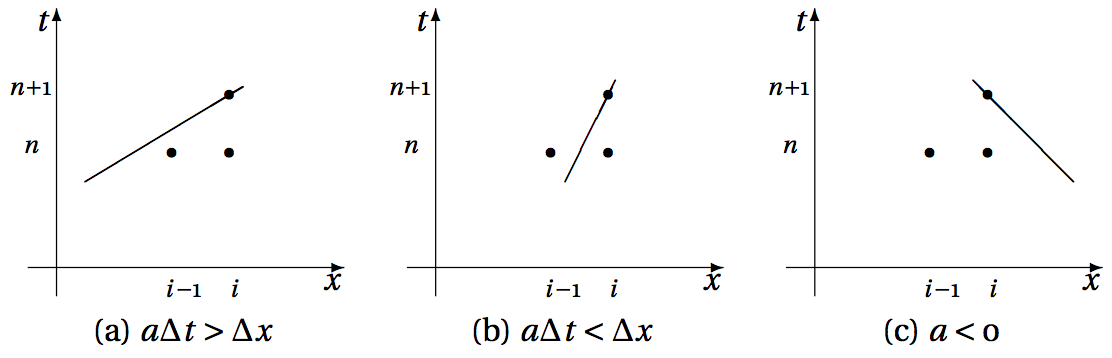
\includegraphics[scale=0.5]{ch3/7}
\captionof{figure}{}
\end{center}

We know that we have a hyperbolic equation that means that there is a characteristic line with slope $\frac{dx}{dt} = a$. We have seen in PDE theory that the solution $u^{n+1}_i$ depends on the solutions that lie on the characteristic passing through it. If we look to case (a) and (c), we see that the numerical domain of dependence (here the segment $[u_{i-1} \ u_i]$) does not include the physical domain of dependence (the characteristic) $\Rightarrow$ unstable, while it is included in the case (b) $\Rightarrow$ stable. This is a \textbf{necessary} stability condition, but not a \textbf{sufficient} condition! Because in the previous scheme, if we take the case $|\sigma| \leq 1 $, the physical domain of dependence is included in the numerical domain, but we have seen that the scheme was unstable.\\

 We can give a more algebraic interpretation: when we look at the numerical scheme 

\begin{equation}
\frac{u_i ^{n+1} - u_i ^n}{\Delta t} + a \frac{u_i ^n - u_{i-1}^n}{\Delta x} = 0 \Rightarrow u_i ^{n+1} = (1-\sigma ) u_i ^n + \sigma u _{i-1}^n
\end{equation}

It is observed that the scheme is stable if $u_i^{n+1}$ is obtained by \textbf{interpolation }of previous time step and unstable if \textbf{extrapolation}. In fact, when $\sigma <1$, we can see in the equation that the coefficients are positive and that the solution is a weighted average of $u^n_{i-1}$ and $u^n_{i}$ and thus lies into the interval $[u^n_{i-1}\ u^n_{i}]$ which rejects solution blow up and oscillations.  If $\sigma < 1$ we have an interpolation and when $\sigma >1, <0$ we have extrapolation. \\

Now if we consider the forward discretization (used for time), we can see that the region of stability goes up to $z=-2$ on \autoref{ch3/3}. The discrete stability condition is therefore $0\leq \sigma \leq 2$. But it is observed that for $1< \sigma \leq 2$ the solution of the upwind scheme blows up rapidly. This has been explained by the fact that first the error is increasing, then it decreases asymptotically for $n\rightarrow \infty$. As we have limited time steps this is unacceptable. 

\subsection{Dissipation and dispersion}
This is in reference to the advection equation 

\begin{equation}
\frac{\D u}{\D t} + a \frac{\D u}{\D x } = 0
\end{equation}

and relate to the behavior of periodic numerical solutions wrt that of the corresponding exact solutions. 

\subsubsection{Properties of the space discretization operator}
These are define with regard to a periodic solution of the closed form $u = f(x-at)$ where in particular $f$ can be a periodic function $u = e^{ik(x-at)} = û(t) e^{ikx}$ where $k$ is the wave number. When we space discretize, we gonna get: 

\begin{equation}
u _ i = \hat{u} (t) e^{ikx_i}\qquad \Rightarrow \frac{d u}{dt} = \lambda ^{(j)} \hat{u}
\end{equation}

where $\lambda$ is an eigenvalue in the discrete spectrum. This $\lambda$ is to be compared with $- i ka $ ($\hat{u} = e^{\lambda^{(j)}t}$). It has a real part and an imaginary part: 

\begin{equation}
\lambda ^{j} = \lambda _r ^{j}+ i\lambda _i^{j}
\end{equation}

If we define $a _{num}$ the numerical wave propagation speed, such that: 

\begin{equation}
\frac{\lambda ^{j}}{-ik_j} = a _{num} ^{j} = a_r ^{j} +  ia_i^{j} \qquad \Rightarrow \hat{u} = e^{\lambda ^{(j)} t} = e^{-ika_r^{(j)}t}e^{ka_i^{(j)}t} = \rho e^{-i\varphi}
\end{equation}

We observe that the error in amplitude wrt the exact solution, called \textbf{dissipative error} is associated with the imaginary part $a_i^{(j)}$ and that the error in phase called \textbf{dispersive error} is related to the real part $a_r^{(j)}$. We define dissipative error $\epsilon_D$ and dispersive error $\epsilon_\varphi$ as: 

\begin{equation}
\epsilon _D = \ln \rho = k_j a_i^{(j)} t = \frac{a_i^{(j)}}{a} k_j \Delta x \underbrace{\frac{at}{\Delta x}}_{t^*}, \qquad \epsilon _\varphi = \frac{\varphi _{num}}{\varphi _{exact}} = \frac{a_r^{(j)}}{a}
\end{equation}

Traditionally we plot $\frac{a _i ^(j)}{a} k_j \Delta x$ (dissipative) vs $\eta= k \Delta x$ and $\frac{a_i^{(j)}}{a}k_j \Delta x= \epsilon _\varphi k_j \Delta x$ (dispersive). For the numerical scheme to be stable the dissipative error must be negative. We will look to two discretization methods. 

\subsubsection{Illustration}
If we do upwind (BW space), then central, knowing the $\lambda$, we have: 

\begin{equation}
\begin{aligned}
\lambda = -\frac{a}{\Delta x} (1 - e^{-i\eta _j}) &= -\frac{a}{\Delta x} (1 - \cos \eta_j) - i \frac{a}{\Delta x} \sin \eta_j\\
&\Rightarrow \frac{a^{(j)}}{a}k_j \Delta x = \frac{i \lambda ^{(j)} \Delta x}{a} = \sin \eta _j - i(1 - \cos \eta _j) \\
\lambda = -i \frac{a}{\Delta x} \sin \eta \qquad &\Rightarrow \frac{a^{(j)}}{a}k_j \Delta x = \frac{i \lambda ^{(j)} \Delta x}{a} = \sin \eta _j
\end{aligned}
\end{equation}

We observe that there is no dispersive part for central discretization (imaginary part). The curves are plotted just below.

\begin{center}
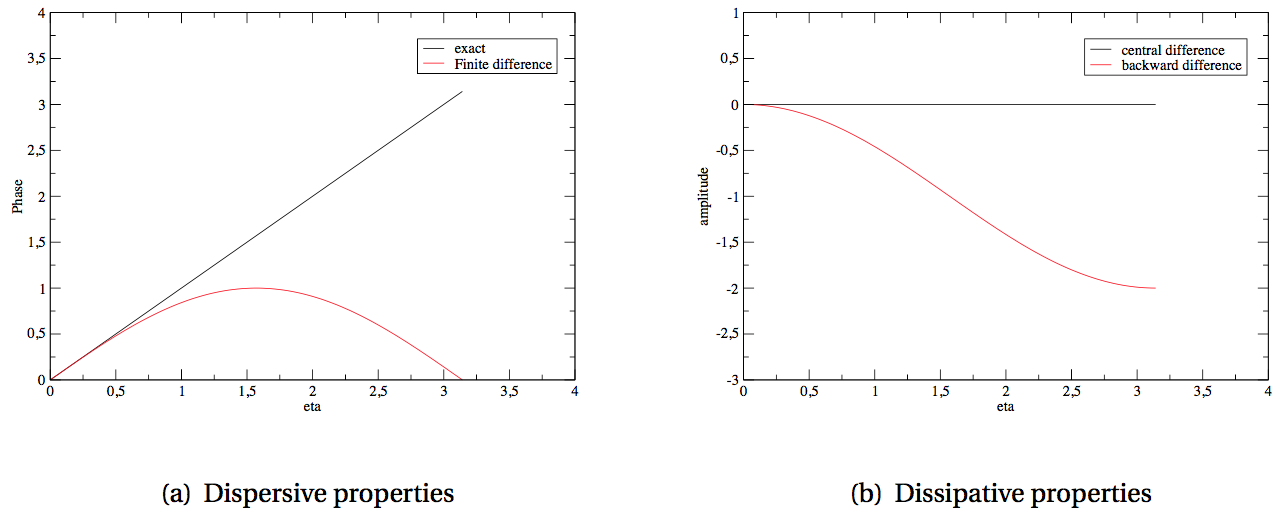
\includegraphics[scale=0.5]{ch3/9}
\captionof{figure}{}
\end{center}

We see indeed that central finite difference is non dissipative and that the backward space is dissipative. Let's concentrate on the dispersive curves, let's recall that the eigenmodes of the waves consists of discrete periodic solutions in space $\nu ^{(j)}_m = \exp (ik_j x_m)$ with wave numbers $k_j = 2\pi j/L, j= 0, \dots, N-1$, so that the erduced wave number is $\eta _j = k_j \Delta x =  2\pi j \Delta x / L = 2\pi j / N$. They vary between 0 and $2 \pi$ or $-\pi, \pi$ (eigenvalues periodic in $\eta$). The numerical solution is thus limited in wavenumber resolution to $\eta \leq \pi$ or $k \leq k_{max} = \pi / \Delta x$.\\

This is similar to the Shannon Nyquist theorem for signal processing where we can only reconstruct frequencies up to $f_s /2$ where $f_s$ is the sampling frequency. In our case, if the sampling wavenumber is $k_s = 2\pi / \Delta x$, the numerical solution can only resolve wavenumbers up to $k = \pi / \Delta x$ and waves with higher wavenumbers than this limit are called \textbf{unresolved}, we need to rescale the mesh. We can observe on the figure that for higher reduced wave numbers $\eta$, the phase lag error increases which leads to numerical errors that are subsequently highlighted. We call these waves \textbf{poorly resolved waves}. For example if we want an accuracy of 5\% in phase, this corresponds to $\eta \leq \pi / 6 \geq 2\pi \Delta x / \lambda \Rightarrow \lambda / \Delta x \geq 12$, we need thus at least 12 points to approximate well this wave. \\

In conclusion, accurately resolved waves should suffer from as low as possible dissipative errors (amplitude), but the dispersive error (phase-lag) should be damped so that the phase lag errors do not pollute the solution. 

\subsubsection{Fully discrete analysis}
As we discretize in time, the time step also contributes to the dissipative and dispersive errors. For periodic solutions in time, the amplification factor $\frac{u^{n+1}_i}{u_i^n}= g(\eta, \sigma) = e^{\lambda _{num}}$ has to be compared with: 

\begin{equation}
\frac{u(x_i , t + \Delta t)}{u (x_i, t)} = e^{\lambda _{exact}\Delta t} = e^{-i k a \Delta t} = e^{- i \eta \sigma}
\end{equation}  

So that the errors are: 

\begin{equation}
\epsilon _D = \ln |g| \mathcal{R}(\lambda _{num}) \Delta t = k a_{num,i} \Delta t=  \frac{a_{num,i}}{a}\eta \sigma \qquad \epsilon _{\varphi} = \frac{arg(g)}{-\eta \sigma} = \frac{a_{num}}{a} 
\end{equation}

We often plot $\epsilon _D/\sigma$ and $\epsilon _\varphi \eta$ as a function of $\eta$. For the upwind scheme we had $g = 1 - \sigma (1 - e^{-i\eta \sigma})$ so that 

\begin{equation}
\epsilon _D / \sigma = \frac{\ln (1 - 2 \sigma (1- \sigma )(1-\cos \eta))}{2\sigma } \qquad \eta _\varphi \eta = \frac{1}{\sigma} \arctan \left( \frac{\sigma \sin \eta }{1 -\sigma (1- \cos \eta)} \right)
\end{equation}

For $\sigma = 1$, we have $\epsilon _D = \epsilon _\varphi = 0$ which means that the scheme becomes exact, the time integrator exactly compensates the dispersive and dissipative errors of the space discretization. This can be understood  when we see that the characteristic passing through the point $i, n+1$ passes through $i-1,n$. This is not possible in practice. For the case $\sigma \rightarrow 0$, we can make a Taylor approximation: 

\begin{equation}
\epsilon _D /\sigma \approx -(1 - \cos \eta) \qquad \epsilon _\varphi \approx \sin \eta
\end{equation}

We recover the result of the semi-discrete analysis, since when $\sigma \rightarrow 0$ the time integration becomes exact. \\

To conclude we will show that the dissipative error is similar to the effect of an artificial diffusion. The advection diffusion equation is: 

\begin{equation}
\frac{\D u}{\D t} + a \frac{\D u }{\D x} = \alpha \frac{\D ^2 u}{\D x^2}
\end{equation}

It admits a periodic solution $u = e^{ik(x-at)}e^{-ak^2 t}$ whose amplification factor is $g_{AD} = e^{-i\eta \sigma}e^{-a \eta ^2 \frac{\Delta t}{\Delta x^2}}$. We have thus applying Taylor approx: 

\begin{equation}
|g|^2 = e^{-a \eta ^2 \frac{\Delta t}{\Delta x^2}} \approx 1 - \frac{a\Delta t}{\Delta x^2} \eta ^2 
\end{equation}

Now also for $\eta \ll 1$ (Taylor), the amplification factor of the upwind scheme is: 

\begin{equation}
g \approx \sqrt{1 - \sigma (1-\sigma )\eta ^2} \approx 1 - \sigma \frac{1-\sigma}{2}\eta ^2
\end{equation}

They have similar form and we can deduce the artificial diffusion term 

\begin{equation}
\alpha _{num} = \frac{\sigma (1-\sigma)}{2}\frac{\Delta x^2}{\Delta t} = \frac{a \Delta x}{2}(1- \sigma)
\end{equation}

We can see that the effects are indeed similar on the figure just below. 

\begin{center}
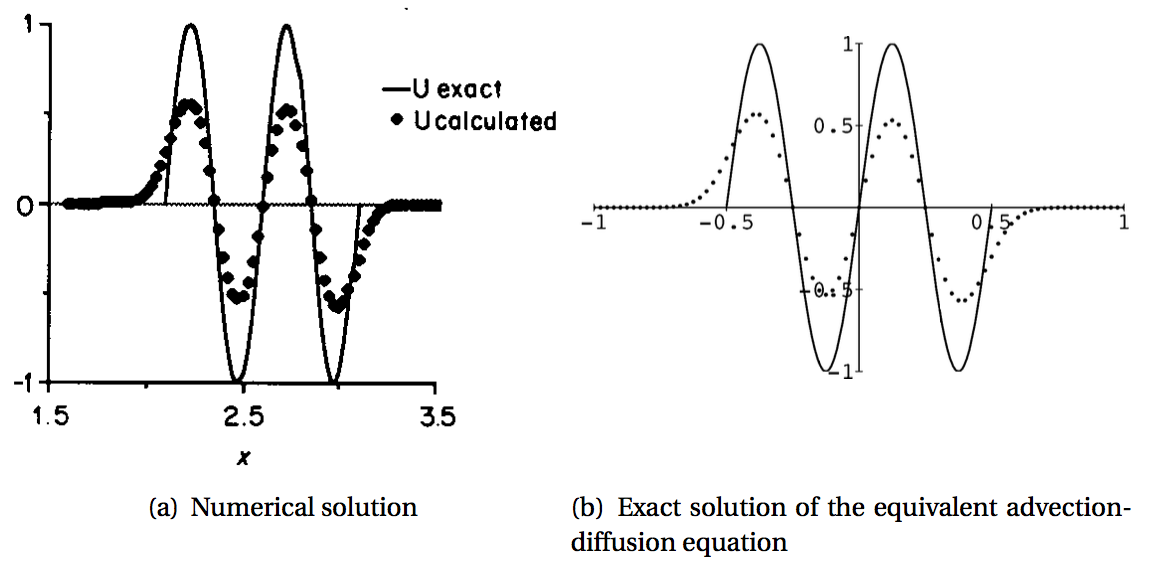
\includegraphics[scale=0.5]{ch3/10}
\captionof{figure}{}
\end{center}

\subsection{Centred schemes: leap-frog, Lax-Friedrichs and Lax-Wendroff}

We started by looking to the FTCS for the transport equation and we saw that it was unstable. We changed space discretization in forward time upwind scheme. This can run to problems with systems, let's show why. First, it is highly dissipative. Second, if we look to the forward time backward space we have: 

\begin{equation}
\frac{\D U}{\D t} + A\frac{\D U}{\D x} \qquad \Rightarrow \frac{U^{n+1}_{i} - U^{n}_{i}}{\Delta t} + A \frac{U^{n}_{i} - U^{n}_{i-1}}{\Delta x} = 0
\end{equation}

If we assume as previously that we have periodic solutions in space, we have: 

\begin{equation}
\begin{aligned}
U_{i-1} = U_i &e^{-i k \Delta x} \qquad \Rightarrow U_i^{n+1} = U_i^n - \frac{A \Delta t}{\Delta x} (1 - e^{-i\eta}) U_i^n \\
&U_i^{n+1} = \underbrace{\left[I - A \frac{\Delta t}{\Delta x} (1 - e^{-i\eta})\right]}_{G} U_i^n
\end{aligned}
\end{equation}

Now we have an \textbf{amplification matrix G} instead of an amplification factor. As the system is supposed to be hyperbolic it has a complete set of eigenvalues and eigenvectors, A is diagonalizable: 

\begin{equation}
A = R\Lambda R^{-1}
\end{equation}

where $\Lambda = diag (\lambda ^{i})$. In addition $I = RR^{-1}$ so that we can rewrite the equation: 

\begin{equation}
\begin{aligned}
&G = R \, \mbox{diag }\left(1 - \lambda ^{(i)}\frac{\Delta t}{\Delta x} (1-e^{-i\eta})\right) R^{-1}\\
&R^{-1}U_i^{n+1} = R^{-1}R \,\mbox{diag} \left(1 - \lambda ^{(i)} \frac{\Delta t}{\Delta x} (1-e^{-i \eta}) \right) R^{-1}U_i^n
\end{aligned}
\end{equation}

We pose $W_i^{n+1} = R^{-1}U_i^{n+1}$, $R^{-1}R = I$ and $W_i^{n} = R^{-1}U_i^{n}$. We can finally write $g^{(i)}$ the eigenvalues of $G$: 

\begin{equation}
W_i^{n+1} = \mbox{diag}\left(g^{(i)}\right) W_i ^n = \sum _{i=1}^m R_i g^{(i)}w_i
\end{equation}

The stability condition can be generalized to: 

\theor{A numerical scheme for the solution of a system of evolution equations is stable iff all eigenvalues of the amplification matrix G are such that their modulus is smaller or equal to unity.

\begin{equation}
|g^{(i)}| =  \left|1 - \lambda ^{(i)} \frac{\Delta t}{\Delta x} (1-e^{-i \eta}) \right| \qquad\Rightarrow 0 \leq \frac{\lambda ^{(i)}\Delta t}{\Delta x} \leq 1
\end{equation}}\ \\

This condition is violated for negative eigenvalues and thus if the eigenvalues are of mixed type (some positive and some negative), the system is unconditionally unstable. This is the case for 1D Euler with eigenvalues of both signs $u-a, u, u+a$, so we cannot use FTBS. We should use then a centered space discretization. 

\subsubsection{Leap-frog scheme}
If we come back to the reason the FTCS doesn't work, we have a region for CS that is purely imaginary and the FT on the left plane of the complex plane has no extend on the imaginary axis. We have already treated the change in space discretization, for time discretization modification we have 3 candidates: the explicit mid-point method (imaginary), Runga Kutta (extension on the real negative and imaginary axis) or implicit schemes (let's forget to the two last and look to the central time). 
The leap-frog consists in using the explicit mid-point, central discretization. For the advection equation we will get: 

\begin{equation}
\frac{u_{i}^{n+1} - u_{i}^{n-1}}{2\Delta t} + a \frac{u_{i+1}^{n} - u_{i-1}^{n}}{2\Delta x} = 0
\end{equation}

First of all we know that the truncation error is more accurate $\mathcal{O}(\Delta t^2, \Delta x^2)$. Since we use the four points around point i, n without using the point itself, it has been called \textbf{Leap-frog scheme}. If we look to the stability via the Fourrier footprint we had a stability region on the imaginary axis going from $-\frac{ia}{\Delta x}$ to $\frac{ia}{\Delta x}$ for the space discretization and for the time discretization is between $-i,i$. Thus the condition of stability is: 

\begin{equation}
\left|\frac{a\Delta t}{\Delta x} \right| = |\sigma | \leq 1
\end{equation}

If we do the one step analysis, we will replace the discretized equation by: 

\begin{equation}
\frac{g u^n_i - \frac{1}{g}u^n_i}{2\Delta t} + a \underbrace{\frac{e^{i\eta}- e^{-i\eta}}{2\Delta x}}_{I\frac{\sin \eta}{\Delta x}} u^n_i = 0 \qquad \Rightarrow g^2 - 1 + 2\frac{a \Delta t}{\Delta x} i \sin \eta g = 0
\end{equation}

For which we get the following solution:

\begin{equation}
g = - i \sigma \sin \eta \pm \sqrt{-\sin ^2 \eta + 1}
\end{equation}

The stability condition is that $1 - \sigma ^2 \sin ^2 \eta \geq 0$ and since $\sin ^2\eta$ is between 1 and 0, we have $\sigma ^2 \leq 1$. We can compute the dissipative and dispersive errors: 

\begin{equation}
\begin{aligned}
&|g|^2 = 1 - \sigma ^2 \sin ^2 \eta + \sigma ^2\sin ^2 \eta = 1 \\
&\Rightarrow arg(g) = \arctan \left(\frac{-\sigma \sin \eta }{1 - \sigma ^2 \sin ^2 \eta} \right) \Rightarrow \epsilon _\varphi = \frac{arg(g)}{-\eta \sigma } = \frac{1}{\eta \sigma } \arctan \frac{\sigma \sin \eta}{1 - \sigma ^2 \sin ^2 \eta}
\end{aligned}
\end{equation}

For $\sigma \rightarrow 0$ the dispersive error becomes $\frac{\sin \eta }{\eta}$, there is no dissipative error, this seems to look perfect. We can see on the figure that we preserve the amplitude of the wave packet. We have dispersive error, phase lag and thus this leeds to spurious oscillations. Poorly resolved high wave number modes are trailing behind the wavepacket on the figure (a). In case of non continuity we have something really poor, showing that non damped poorly resolved modes can affect the solution very badly. We can show these oscillations, let's take the discretized equation: 

\begin{equation}
u^{n+1}_i = u^{n-1}_i - \sigma u_{i+1}^n + \sigma u_{i-1}^n
\end{equation}

Where we have a negative term with sigma, the reason of oscillations. 

\begin{center}
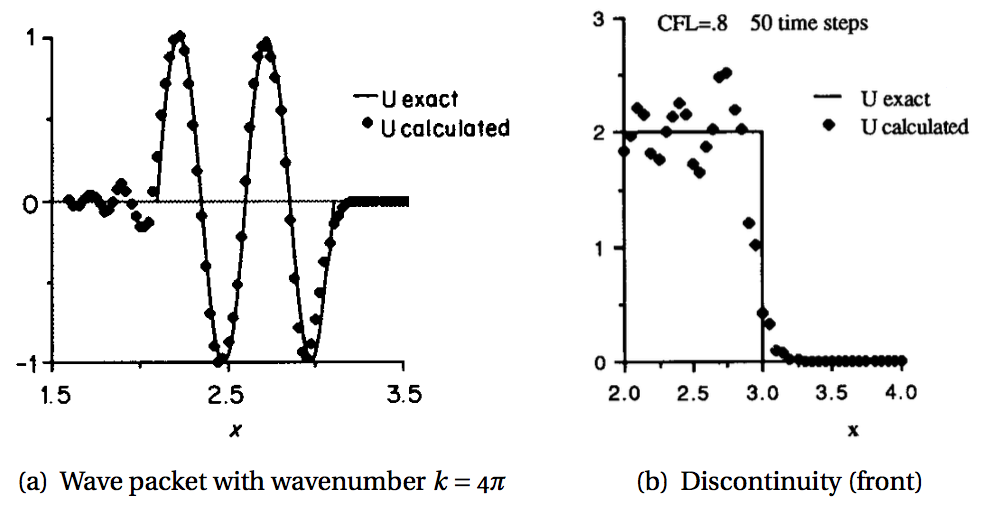
\includegraphics[scale=0.5]{ch3/11}
\captionof{figure}{}
\end{center}

\subsubsection{Lax-Friedrischs scheme}
We want to manipulate the FTCS to stabilize it and we want to replace the $u_i^n$ in the time discretization by an average of the two neighbors $\frac{1}{2} (u_{i-1}^n + u_{i+1}^n)$, this gives: 

\begin{equation}
\frac{u_i ^{n+1} - \frac{1}{2}(u_{i-1}^n + u_{i+1 ^n})}{\Delta t} + a \frac{u_{i+1}^n - u_{i-1}^n}{2\Delta x} = 0
\end{equation}

The truncation error of this is $TE = \mathcal{O} (\Delta t, \Delta x^2 / \Delta t)$. We see that the two discretizations are not independent and are coupled due to the neighboring average, this does not allow us to make a separate region of dependance analysis. We can rewrite the scheme as: 

\begin{equation}
u_i^{n+1} = \frac{1}{2} (1 + \sigma )u_{i-1}^n + \frac{1}{2} (1- \sigma ) u_{i+1}^n
\end{equation}

For this to be stable we need $-1 \leq \sigma \leq 1$ so that both coefficients are >0 to have stability and non oscillatory solution. We can check this by Fourrier footprint: 

\begin{equation}
g = \frac{1}{2} (1+\sigma) e^{-i\eta} + \frac{1}{2}(1-\sigma) e^{i\eta} = \cos \eta - \sigma i \sin \eta \qquad
\begin{aligned}
&\Rightarrow |g|^2= \cos ^2 \eta + \sigma ^2 \sin ^2 \eta \\
&= 1 - (1 - \sigma ^2)\sin ^2\eta \leq 1 \Rightarrow \sigma ^2 \leq 1
\end{aligned}
 \end{equation}
 
We can compute the arg(g): 
 
\begin{equation}
\begin{aligned}
&arg(g) = \arctan \frac{-\sigma \sin \eta}{\cos \eta} = \arctan (-\sigma \tan \eta) \\
\Rightarrow &\epsilon _\varphi = \frac{arg(g)}{-\eta \sigma} = \frac{\arctan (\sigma \tan \eta)}{\sigma \eta} \rightarrow \frac{\tan \eta}{\eta} \quad \mbox{for } \sigma \rightarrow 0
\end{aligned}
\end{equation}

It is dissipative (stronger damping than upwind scheme) but there is no oscillation as can be seen in the case of the front. Can we assemble the two schemes? We will see it in the next method.

\begin{center}
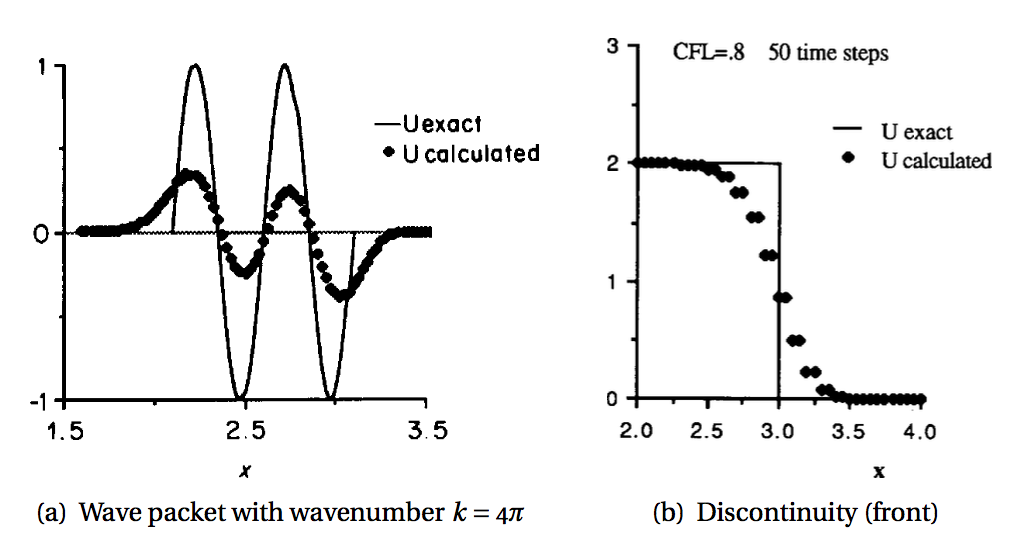
\includegraphics[scale=0.5]{ch3/12}
\captionof{figure}{}
\end{center}

\subsubsection{Lax-Wendroff scheme}
It consists in one step of Friedrichs and one step of Leap-Frog. We will generate using Fridrichs the points $u^(n+1)_{i-1}, u^(n+1)_{i+1}$  and use the Leap to get from these two the point $u_{i}^{n+2}$. Mathematically, we use the Friedrichs method: 

\begin{equation}
u_i^{n+1} = \frac{1}{2}(1+\sigma )u_{i-1}^n + \frac{1}{2}(1-\sigma) u_{i+1}^n
\end{equation}

Then we get the two points 

\begin{equation}
u_{i-1}^{n+1} = \frac{1}{2}(1+\sigma )u_{i-2}^n + \frac{1}{2}(1-\sigma) u_{i}^n\qquad 
u_{i+1}^{n+1} = \frac{1}{2}(1+\sigma )u_{i}^n + \frac{1}{2}(1-\sigma) u_{i+2}^n
\end{equation}

Then we will just shift the n indices +1 in central central schemes to make appear the $n+1$ on $u$: 

\begin{equation}
\frac{u_i^{n+2} - u_i^n}{2\Delta t} + a \frac{\frac{1}{2}(1+\sigma)u_i^{n} + \frac{1}{2}(1-\sigma)u_{i+2}^n-\left(\frac{1}{2}(1+\sigma)u_{i-2}^n + \frac{1}{2}(1-\sigma)u_i^n \right)}{2\Delta x}
\end{equation}

By considering the mesh regrouping two squares in one

\begin{equation}
\frac{u_i^{n+1} - u_i^n}{2\Delta t} + a \frac{\frac{1}{2}(1+\sigma)u_i^{n} + \frac{1}{2}(1-\sigma)u_{i+1}^n-\left(\frac{1}{2}(1+\sigma)u_{i-1}^n + \frac{1}{2}(1-\sigma)u_i^n \right)}{2\Delta x}
\end{equation}

Then we can rewrite

\begin{equation}
\begin{aligned}
&u_i^{n+1} - u_i ^n + \sigma \underbrace{\left[ \frac{1}{2}(1-\sigma)u_{i+1}^n + \sigma u_i ^n - \frac{1}{2} (1+\sigma) u _{i-1}^n \right]}_{\frac{u_{i+1}^n- u _{i-1}}{2}^n - \sigma \frac{u_{i+1}^n - 2u_i ^n + u_{i-1}^n}{2}} = 0\\
&\Rightarrow u_i^{n+1} = u_i^n - \sigma \frac{u_{i+1}^n - u_{i-1}^n}{2} + \sigma ^2 \frac{u_{i+1}^n - 2u_i^n + u_{i-1}^n}{2}
\end{aligned}
\end{equation}

\theor{
\textbf{MIGUEL CAN YOU DO HERE PLEASE}\\
If we do a Taylor expansion 

\begin{equation}
u_{i}^{n+1} =  u_i^n + \Delta t \left. \frac{\D u}{\D t} \right|^n_i + \frac{\Delta t^2}{2} \left. \frac{\D ^2 u}{\D t^2} \right| ^n_i  + \mathcal{O}(\Delta t^3)
\end{equation}

We know from the advection $\frac{\D u}{\D t} + a \frac{\D u}{\D x} = 0$ equation that 

\begin{equation}
\frac{\D ^2 u}{\D t^2} = \frac{\D}{\D t}\left(\frac{\D u}{\D t} \right) = \frac{\D }{\D t} \left( -a \frac{\D u}{\D x} \right) = -a \frac{\D}{\D x} \left( \frac{\D u }{\D t} \right) = a^2 \frac{\D^2 u }{\D x^2}
\end{equation}

If we come back to the Taylor we can replace the first derivative and the second by respectively: 

\begin{equation}
-a \frac{\D u}{\D x} \approx -a \frac{u_{i+1}-u_{i-1}}{2\Delta x} + \mathcal{O}(\Delta x^2) \qquad a^2\frac{\D ^2 u}{\D x^2} \approx a^2 \frac{u_{i+1}^n}{•}
\end{equation}

Not had the time to copy ...
}

Stability analysis: 

\begin{equation}
\begin{aligned}
g &= 1 - \sigma \frac{e^{i\eta} - e^{-i\eta}}{2} + \frac{\sigma ^2}{2} (e^{i\eta} + e^{-i\eta}-2) = 1 - i \sigma \sin \eta + \sigma ^2 (\cos \eta -1)\\
|g|^2 &= [1 - \sigma ^2 (1 -\cos \eta)]^2 +\sigma^2 \sin ^2 \eta = 1 - 2 \sigma ^2 (1- \cos \eta) + \sigma ^4 (1 - \cos \eta)^2 \\
&+ \sigma ^2 (1-\cos ^2\eta)= 1 - (1 -\cos \eta) [2- (1 + \cos \eta) - \sigma ^2 (1 - \cos \eta)] \\
 &= 1 - \sigma ^2 (1-\cos \eta ) [1 - \cos \eta - \sigma ^2 (1- \cos \eta)] = 1 - \sigma ^2 (1- \sigma ^2) (1 - \cos \eta )^2 \leq 1
\end{aligned}
\end{equation}

Since the squares are positive, we have $1 - \sigma ^2 \geq 0\Leftrightarrow \sigma ^2 \leq 1$. Studying the dissipative error, $1 - \cos \eta = 2\sin ^2 (\eta /2)$ so that: 

\begin{equation}
\epsilon _D = \ln(g) = \frac{1}{2}\ln (1-4\sigma ^4\frac{\eta}{2}(1-\sigma ^2))
\end{equation}

we have a $4 \sin ^4 (\eta /2)$ for the dissipation so that the $^4$ term being much smaller than the previous case, reduces the damping in the amplitude. Now if we do the argument: 

\begin{equation}
arg(g) = - \arctan \frac{\sigma \sin \eta }{1 - \sigma ^2 (1 - \cos \eta)} \Rightarrow \epsilon _\varphi = \frac{1}{\eta \sigma} \arctan \frac{\sigma \sin \eta}{1- \sigma ^2 (1- \cos \eta)}
\end{equation} 

For $\sigma \rightarrow 0: \epsilon \varphi = \frac{\sin \eta}{\eta}$. If we look to the numerical solution on the figure, we see that for the small wave number, there is very little damping. There is much less spurious oscillations than before but they are still present. It is easy to see why there is oscillations, because when $-1 \leq \sigma\leq 0$ and $0\leq \sigma \leq 1$ there is one negative term if we rewrite in the form: 

\begin{equation}
u_i^{n+1} = \frac{1}{2}(\sigma ^2 - \sigma)u^n_{i+1} + (1-\sigma ^2)u_i^{n}+ \frac{1}{2}(\sigma ^2 + \sigma) u_{i-1}^n
\end{equation}

\begin{center}
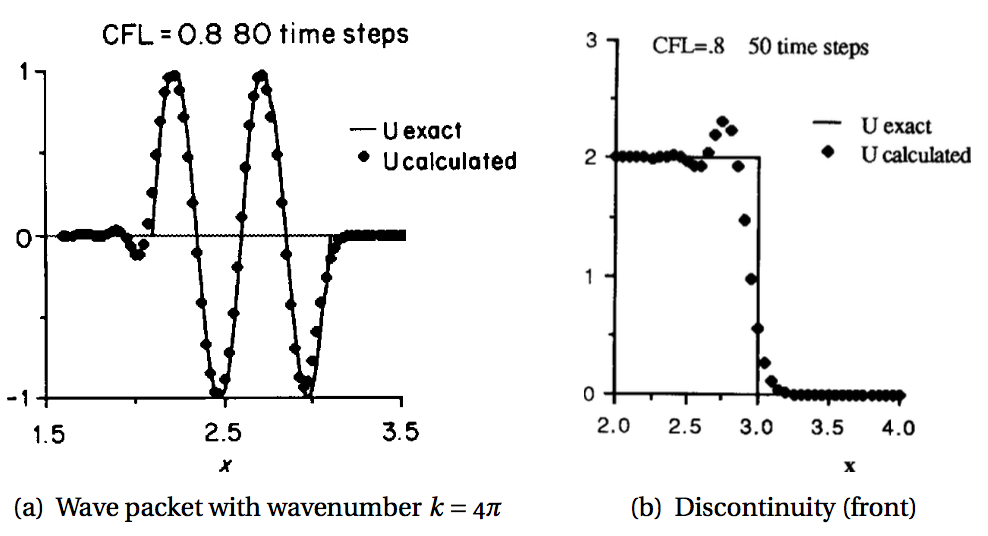
\includegraphics[scale=0.5]{ch3/13}
\captionof{figure}{}
\end{center}


\subsection{Implicit schemes}
We are still dealing with hyperbolic equations. We need to have a part of the imaginary axis, this is what we are going to look now. Remember that when we are doing central space we have a footprint $[-a/\Delta x, a/\Delta x]$ and the Fourrier footprint of the backward time was a circle centered in the positive real axis. Let's test that: 

\begin{equation}
\frac{du_i}{dt} + a \frac{u_{i-1}-u_{i+1}}{2\Delta x} = 0
\end{equation}

Let's first analyze the expression of FT and BT: 

\begin{equation}
\frac{u^{n+1}- u^n}{\Delta t} = f(u^n) \qquad \frac{u^{n}- u^{n-1}}{\Delta t} = f(u^n) \Rightarrow FT = f(u^{n+1})\ BT
\end{equation}

General 1 step: 

\begin{equation}
\frac{u^{n+1}-u^n}{\Delta t} = \theta f(u^{n+1}) + (1-\theta)f(u^n)
\end{equation}

So that the first equation becomes now:

\begin{equation}
\frac{u_i^{n+1}-u_i^n}{\Delta t} + \frac{a}{2\Delta x} \left[ \theta (u_{i+1}^{n+1}-u_{i-1}^{n+1})+ (1-\theta )(u_{i+1}^n - u_{i-1}^n)  \right) = 0 \qquad \frac{du}{dt} = f(u)
\end{equation}

Stability condition (replace eta)



\begin{equation}
g(1+i \sigma \theta \sin \eta ) = 1- i\sigma (1-\theta)\sin \eta \qquad |g|^2 = \frac{1+\nu ^2 (1-\theta)^2 \sin ^2\eta)}{1+\sigma ^2\theta ^2\sin ^2\eta} \leq 1 \qquad (1-\theta)^2 \leq \theta ^2 \Leftrightarrow 1-\theta \leq \theta \Leftrightarrow \theta \geq 1/2
\end{equation}

For the stability analysis:

\begin{equation}
\frac{u^{n+1}-u^n}{\Delta t} = q [\theta u^{n+1}+ (1-\theta)u^n]\qquad g-1 = z[\theta g +(1-\theta)] \Rightarrow g(1-\theta z) \leq 1+(1-\theta)z \qquad |g| = \frac{|1+(1-\theta)z|}{|1-\theta z|} \qquad z=x+iy \Rightarrow [1+(1-\theta)x]^2 + (1-\theta)^2 \eta ^2 \leq (1-\theta x)^2 + \theta ^2 \eta ^2
\end{equation}

This is a circle etc see syllabus

The general one step rewrites: 
\begin{equation}
u^{n+1} = u^n + \Delta t [\theta f(u^{n+1}) + (1-\theta) f(u^n)]
\end{equation}

If we take 1/2 and 1/2 as coefficients, the method is trapezoidal non dissipative. Let's look to the question of spurious oscillations or not. Reads the syllabus. 

We have a linear combination of terms so that we have a tridiagonal system of equation. They are easily solved and are inexpensive in memory. This is for 1D but it becomes very hard with more. The analysis for the oscillations is more complicated than before, we find that 

\begin{equation}
U^{n+1}= K^{-1}AU^n = CU^n
\end{equation}

The sum of the coefficient should be 1 ... 


\subsection{Upwind schemes for systems of equations with characteristic speeds of mixed signs}
We mentioned that it was impossible to use fully biased schemes for mixed sign because the BS is unstable for all the eigenvalues negative and conversely the FT was for the positive eigenvalues. So one way to get around the problem is to use characteristic decomposition. The eigenvalues are real since we are hyperbolic. The model linear problem is: 

\begin{equation}
\frac{\D U}{\D t}+ A\frac{\D U}{\D x} = 0 \qquad A = R\Lambda R^{-1}
\end{equation}

If we multiply this by $R^{-1}$: 

\begin{equation}
R^{-1}\frac{\D U}{\D t}+ R^{-1}A\frac{\D U}{\D x} = 0 = \frac{\D}{\D t} (\underbrace{R^{-1}U}_{W}) + \Lambda \frac{\D}{\D x} (\underbrace{R^{-1}U}_{W})
\end{equation}

We have thus that in equation form: 

\begin{equation}
w_{j,i}^{n+1}= w_{j,i}^{n} + \frac{\Delta t}{\Delta x} \lambda ^{(j)}(w_{j,i}^{n} - w_{j,i+1}^{n}) \qquad \lambda ^{(j)}>0
\end{equation}

and also 

\begin{equation}
w_{j,i}^{n+1}= w_{j,i}^{n} + \frac{\Delta t}{\Delta x} \lambda ^{(j)}(w_{j,i+1}^{n} - w_{j,i}^{n}) \qquad \lambda ^{(j)}<0
\end{equation}

This is called the CIR scheme. This becomes: 

\begin{equation}
\frac{\D w}{\D x} \rightarrow \begin{array}{c}
\lambda \frac{w_i - w_{i-1}}{\Delta x} \quad \lambda > 0\\
\lambda \frac{w_{i-1} - w_{i}}{\Delta x} \quad \lambda < 0
\end{array}
\qquad \lambda \frac{\D w}{\D x} \approx \lambda \frac{w_{i+1}-w_{i-1}}{2\Delta x} - |\lambda|\frac{w_{i+1}-2w_i + w_{i-1}}{2\Delta x} 
\end{equation}

This equation can be interpreted as a central scheme with a bit of diffusion since the second term is a second derivative discretization. This can be written: 

\begin{equation}
A \frac{\D U}{\D x} \approx A\frac{U_{i+1}-U_{i-1}}{2\Delta x} - |A|\frac{U_{i+1}-2U_i + U_{i-1}}{2\Delta x} 
\end{equation}

where we define $|A| = R \, |\mbox{diag}(\lambda ^{(j)})| R^{-1}$.

\subsubsection{Conservative discretization - shock capturing}
read

Page 112

Leap Friedrich: 

\begin{equation}
\frac{U_i^{n+1/2}-\frac{1}{2}U_{i+1}^n+U_{i-1}^n}{\Delta t+2} + \frac{F_{i+1/2}^n-F^n_{i-1/2}}{\Delta x}=0 
\end{equation}

And the leap frog 

\begin{equation}
\frac{U_i^{n+1}-U_i^n}{\Delta t}+ \frac{F^{n+1/2}_{i+1/2}-F_{i-1/2}^{n+1/2}}{\Delta x} = 0
\end{equation}

Implicit schemes p 113
We are considering: 

\begin{equation}
\frac{\D u}{\D t }+ \frac{\D f(u)}{\D x} 
\end{equation}

Using implicit time and central space: 

\begin{equation}
\frac{u^{n+1}_i-u_i^n}{\Delta t} + \frac{1}{2\Delta x} [\theta (f_{i+1}^{n+1}-f_{i-1}^{n+1})+(1-\theta) (f_{i+1}^n)-f^n_{i-1}]
\end{equation}

It is too expensive since it is not a linear equation. A way to make it cheaper is to make as described. 

\section{Numerical schemes for parabolic equations}
The model equation is: 

\begin{equation}
\frac{\D u}{\D t} = \alpha \frac{\D ^2 u}{\D x^2}
\end{equation}

Here FTCS works because the region of stability of both are imbricated so that we need: 

\begin{equation}
\frac{-4\alpha \Delta t}{\Delta x^2} > -2 \qquad \frac{\alpha \Delta }{\Delta x^2}<1/2
\end{equation}

Details are not important on page 111
